\section{Einführung}

\subsection{Vorstellung}

\addtocounter{framenumber}{1}
\begin{frame}[standout]
    \LARGE
    Vorstellungsrunde :)
    \pnote{Selbst: Informatik MSc., letztes Jahr großes Interesse, jetzt Workshop}
\end{frame}


\subsection{Motivation}

% start with something familiar?

\addtocounter{framenumber}{1}
\begin{frame}[standout]
    \LARGE
    Was erwartest du dir \\
    von diesem Workshop?
    \pnote{Sammeln, und in Conclusion eintragen!}
\end{frame}


\begin{frame}[c]{Situation}
    \Large
    \begin{itemize}[<+(1)->]
        \item Man hat etwas vor
        \item Es kommt etwas dazwischen
        \item Ziel wird vergessen
    \end{itemize}
\end{frame}

\begin{frame}[c]{Ziele des Workshops}
    \large
    \begin{itemize}[<+(1)->]
        \item Jeder schreibt seine Ziele auf
        \item Jeder macht sich sehr genaue Gedanken über seine Ziele
        \item Jeder sucht sich eine Vertrauensperson, um den Fortschritt regelmäßig zu teilen
    \end{itemize}
\end{frame}




% Forschung: 149/267 Teilnehmer
% Zufällig gruppe zugewiesen
% - gruppe 1 hat sich über die Ziele gedanken gemacht
%   rate that goal on the following dimensions: Difficulty, Importance, the
%   extent to which they had the Skills & Resources to accomplish the goal,
%   their Commitment and Motivation to the goal, whether or not they had
%   Pursued this goal before and if so their Prior Success.
% jede gruppe hat auch das getan, was die gruppe davor getan hat
% - Participants in Groups 2-5 were asked to write (type into the online survey)
% their goals and then to rate their goals on the same dimensions.
% - Group 3 was also asked to formulate action commitments.
% - Group 4 was asked to formulate action commitments and send their goals and
% action commitments to a supportive friend.
% - Group 5 was asked to formulate action commitments and send their goals,
% action commitments and weekly progress reports to a supportive friend.

\begin{frame}[c]{Stand der Forschung}
    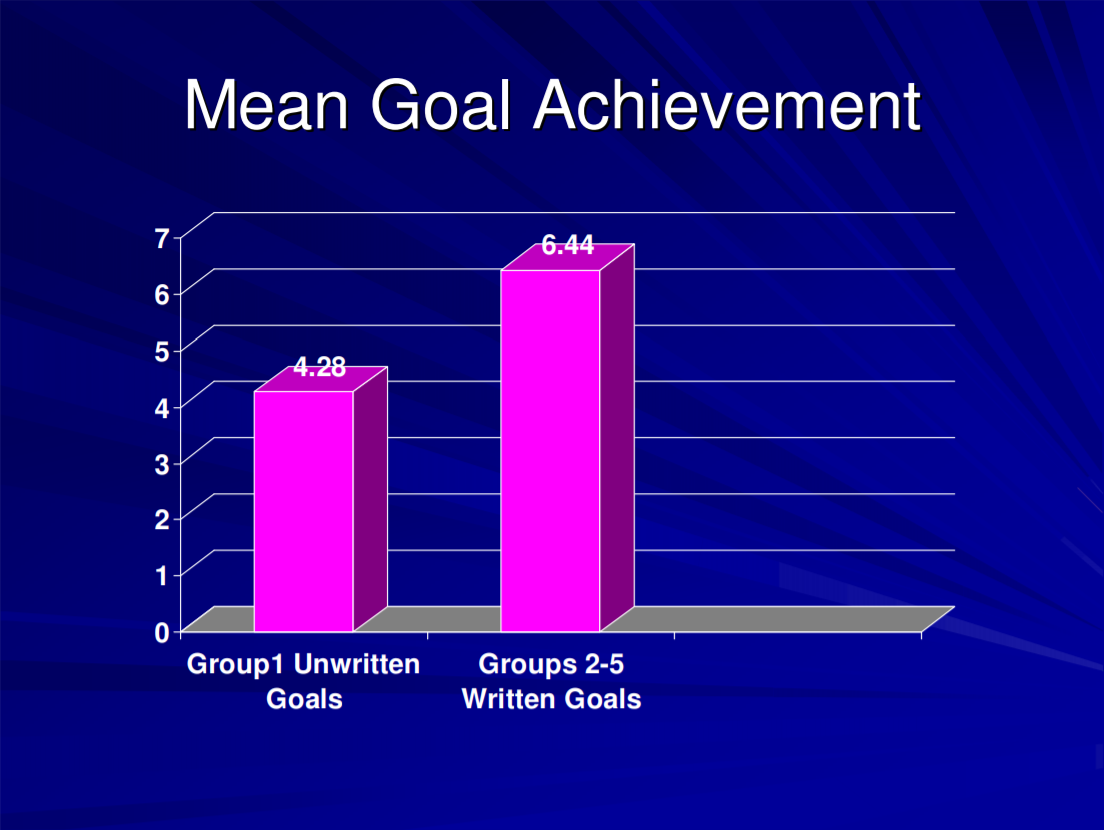
\includegraphics[height=0.8\textheight]{goal_achievement_two} \\
    Nach \cite{better-goals-2} hilft es, seine Ziele aufzuschreiben.
\end{frame}

\begin{frame}[c]{Stand der Forschung II}
    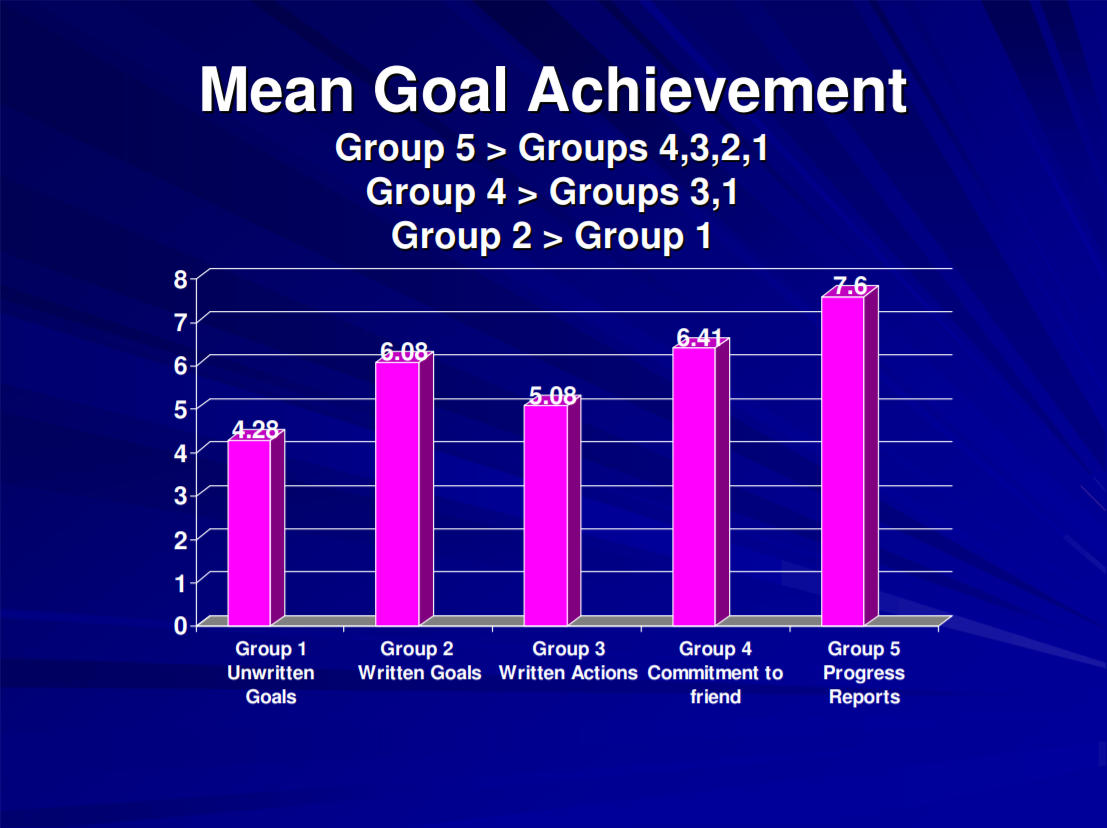
\includegraphics[height=0.8\textheight]{goal_achievement_all} \\
    Außerdem gibt es weitere helfende Maßnahmen \cite{better-goals-2}.
    \pnote{
    Forschung: 149/267 Teilnehmer
    Zufällig Gruppe zugewiesen
    - Gruppe 1 hat sich über die Ziele Gedanken gemacht
      rate that goal on the following dimensions: Difficulty, Importance, the
      extent to which they had the Skills and Resources to accomplish the goal,
      their Commitment and Motivation to the goal, whether or not they had
      Pursued this goal before and if so their Prior Success.
    jede Gruppe hat auch das getan, was die Gruppe davor getan hat
    - Participants in Groups 2-5 were asked to write (type into the online survey)
    their goals and then to rate their goals on the same dimensions.
    - Group 3 was also asked to formulate action commitments.
    - Group 4 was asked to formulate action commitments and send their goals and
    action commitments to a supportive friend.
    - Group 5 was asked to formulate action commitments and send their goals,
    action commitments and weekly progress reports to a supportive friend.
    }


\end{frame}



\subsection{Ablauf}


\begin{frame}[c]{Ablauf}
    \begin{itemize}[<+(1)->]
        \item Ich gebe ein Thema/Aufgabe vor
        \item Erkläre, warum man das machen will
        \item Was die Erfolgskriterien sind
        \item Jeder bearbeitet die Aufgabe
        \item Jeder der will, teilt seine Ergebnisse/Erfolge
        \item Repeat
    \end{itemize}
    \pnote{Frage: Besser zu zweit in Breakout-Rooms?}
\end{frame}


\begin{frame}[c]{Inhalt}
    \large
    \begin{itemize}[<+(1)->]
        \item Persönliche Anekdoten
        \item Wissenschaftliche Ergebnisse
        \item Funktioniert vielleicht nicht für dich!
    \end{itemize}
    \pnote{Es sind auch teile dabei, die für mich nicht gut funktionieren!}
\end{frame}


\begin{frame}[c]{Vorbereitung}
    \begin{itemize}[<+(1)->]
        \item Papier und Stift bereit legen
        \item Platzhalter für Ideen anlegen
        \item Platz für Markierungen lassen
        \item (Eventuell: Ausführung \cite{longtermplans-post} oder PDF \cite{longtermplans-pdf} in einem Tab öffnen)
    \end{itemize}
    \pause
    PDF: \url{https://github.com/fkarg/things-to-talk-about/blob/master/longtermplans/main_handout.pdf}
    \pnote{Links auch nochmal direkt schicken}
\end{frame}


\begin{frame}[c]{Agenda}
    \large
    \begin{itemize}[<+(1)->]
        \item Inhalt: Hängt von euch ab!
        \item Format: Interaktiv!
        \item Immer: Listen schreiben!
    \end{itemize}
\end{frame}


% \begin{frame}[c]{Themen}
%     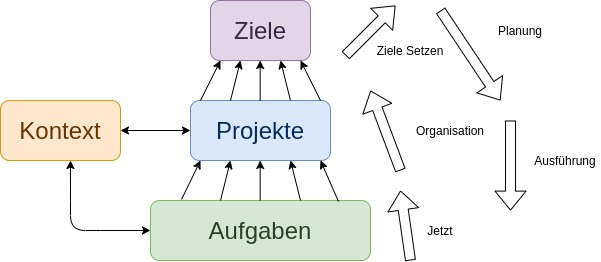
\includegraphics[width=\textwidth]{Ziele_Aufgaben}
% \end{frame}
%
%
% \begin{frame}[c]{Thema: Jetzt}
%     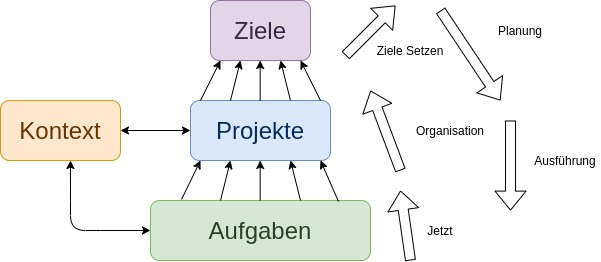
\includegraphics[width=\textwidth]{Ziele_Aufgaben}
% \end{frame}
